\chapter{函数的极限和连续函数的性质}

\section{函数的极限}
\subsection{函数极限的概念}

在第四册下,我们研究了数列的极限,数列是一种特殊的函数,这里的自变数$n$取自然数列$1, 2, 3,\ldots,n,\ldots$的值,现在我们来研究更一般的情形,即函数$f(x)$随$x$连续变化而变化的情形,下面转到一般函数的极限。

\begin{blk}{定义1}
    如果$x$通过任何一个无限增大的数列$\{x_n\}$, 对应的函数值数列
$f (x_1 ) ,f (x_2) , \ldots,f (x_n ) ,\ldots$
都以定数$\ell$为它的极限,就说函数$f(x)$, 当$x\to +\infty$时,以$\ell$为极限,记作
\begin{equation}
    \lim_{x\to+\infty}f(x)=\ell\qquad \text{或}\qquad f(x)\to \ell\quad (x\to +\infty)
\end{equation}
\end{blk}
 
从几何上看,极限式(1.1)表示随着$x$无限增大,曲线$y=f(x)$以直线$\ell$为渐近线(图1.1)。
\begin{figure}[htp]
    \centering
    
    \caption{}
\end{figure}

类似地,可以定义函数极限$\Lim_{x\to -\infty} f(x)=\ell$, 这时,变量
$x$通过代数值无限地变小,而绝对值无限地增大的任何一个数列$\{x_n\}$。

如果函数$f(x)$当$x\to+\infty$和$x\to-\infty$时,都以定值为极限,就说$f(x)$当$x\to \infty$时,以定值$\ell$为极限,记作$\Lim_{x\to\infty}f(x)=\ell$, 或者$f(x)\to \ell\; (x\to\infty)$。

\begin{example}
    证明$\Lim_{x\to\infty}\frac{1}{x}=0$
\end{example}

\begin{proof}
任何数列$\{x_n\}$的值$x_1,x_2,\ldots,x_n,\ldots$趋向于$+\infty$或$-\infty$时,对应的函数数列
\[\frac{1}{x_1},\frac{1}{x_2},\ldots, \frac{1}{x_n},\ldots\]
的绝对值$\left|\frac{1}{x_n}\right|$便趋向于零,即
    \[\lim_{n\to\infty}\left|\frac{1}{x_n}\right|=0\]
    从而$\Lim_{x\to\infty}\frac{1}{x}=0$
\end{proof}

\begin{example}
证明函数$\sin x$, 当$x\to\infty$时,没有极限.
\end{example}

\begin{proof}
令自变量$x$取数列$x_n=-\frac{\pi}{2}+2n\pi\quad (n=1,2,3,\ldots)$的值趋向$+\infty$,则对应的函数值数列
\[\begin{split}
    \sin x_n&=\sin\left(-\frac{\pi}{2}+2n\pi\right)\\
&=\sin\left(-\frac{\pi}{2}\right) =-1 \qquad (n=1, 2, 3, \ldots) .
\end{split}\]
恒取定值$-1$, 于是
\[\lim_{n\to\infty} \sin x_n=\lim_{n\to\infty} \sin \left(-\frac{\pi}{2}+2n\pi\right)=-1\]

再令自变量$x$取数列
\[x_n=\frac{\pi}{2}+2n\pi\qquad  (n=1, 2, 3, \ldots )\]
的值趋向于$+\infty$, 则对应的函数值数列
\[\sin x_n =\sin\left(\frac{\pi}{2}+2n\pi\right) =1\qquad  (n=1, 2, 3, \ldots)\]
恒取定值1,于是
\[\lim_{n\to\infty} \sin x_n=\lim_{n\to\infty} \sin\left(\frac{\pi}{2}+2n\pi\right) =1\]
由于$x$取趋向$+\infty$的两个不同数列时,$y=\sin x$可以有不同的极限,因此
$\Lim_{x\to\infty} \sin x$不存在。
\end{proof}

\begin{blk}{定义2}
 设函数$f(x)$在点$a$附近有定义(但在$x=a$时,
可以没有定义),如果当自变量$x$不论通过怎样一个以$a$为极限但始终不等于$a$的数列$\{x_n\}$, 对应的函数值数列$f (x_1) ,f (x_2) , \ldots,f(x_n ) ,\ldots$
总有极限$\ell$, 就说:

当$x$趋近于$a$时,$f(x)$以$\ell$为极限,记作
\begin{equation}
   \lim_{x\to a}f(x)=\ell,\qquad \text{或}\qquad f(x)\to \ell\quad (x\to a) 
\end{equation}
\end{blk}

极限式(1.2)的几何意义如图1.2所示:当$x$无限地靠近$a$,但总不能等于$a$时,曲线$y=f(x)$上的点$(x,f(x))$无限地近$(a,\ell)$点.

\begin{figure}[htp]
    \centering
    
    \caption{}
\end{figure}

初学的人常常要问:为什么在定义中谈到$x$趋近于$a$时,要限制$x$始终不等于$a$呢?这是因为我们关心的是函数$f(x)$在$a$附近的变化趋势,它和函数$f(x)$在
$x=a$这一点的值没有什么必然关系,这也就是说,无论$f(x)$在点$a$取什么值甚至没有定义,都不影响在这一点的极限的存在和极限值。

\begin{example}
设$f(x)=\frac{3}{4}\cdot \frac{x^2-1}{x-1}$,$x\in(-\infty,1)\cup(1,+\infty)$,求$\Lim_{x\to 1}f(x)$
\end{example}

\begin{solution}
    $f(x)=\frac{3}{4}\cdot \frac{x^2-1}{x-1}$在$x=1$时无意义,因为那时
    分母就变成零,因此,这里没有函数值$f(1)$, 曲线$y=f(x)$也没有相应于横坐标为1的那个点,但是让$x$任意地趋近于1是完全可以的,若$x\ne 1$, 则有
  \[  f (x) =\frac{3}{4}\cdot  \frac{(x-1)(x+1)}{x-1}=\frac{3}{4}(x+1)\]
  因此,不论$x$通过怎样一个以1为极限的数列$\{x_n\}$, 对于相应的数列$\{f(x_n)\}$, 我们都有
  \[\lim_{x_n\to 1} f (x_n) =\frac{3}{4} (1+1) =\frac{3}{2}\]

    从几何上看,曲线$y=f(x)$除去点$\left(1,1\frac{1}{2}\right)$外是与直线$y=\frac{3}{4}(x+1)$一致的,唯独在那一点,曲线有个空隙,而在$x=1$的邻近的点只要充分接近于点1, 所对应的函数值与$\frac{3}{2}$的差的绝对值可以任意小,如图1.3。
\end{solution}
    
\begin{figure}[htp]
    \centering
\begin{tikzpicture}[>=latex]
    \draw[->](-3,0)--(5,0)node[right]{$x$};
    \draw[->](0,-1.5)--(0,4.5)node[right]{$y$};
\foreach \x in {1,2,3}
{
    \draw(0,\x)node[left]{$\x$}--(.1,\x);
    \draw(\x,0)node[below]{$\x$}--(\x,.1);
}
\node at (.25,-.25){$O$};
\draw[dashed](0,1.5)--(1,1.5)--(1,0);
\draw[domain=-2:4, samples=10, very thick]plot(\x, {0.75*(\x+1)});
\draw(1,1.5)[fill=white]  circle(1.5pt) node[right]{$\left(1,1\tfrac{1}{2}\right)$};
\node at (3.25,3)[right]{$y=\frac{3}{4}\cdot \frac{x^2-1}{x-1}$};
\end{tikzpicture}
    \caption{}
\end{figure}

\begin{example}
证明当$x\to 0$时,函数$f(x)=\sin\frac{1}{x}$没有极限。
\end{example}

\begin{proof}
函数$f(x)=\sin\frac{1}{x}$对于一切$x\ne 0$的值有定义,因此这个函数在点$x=0$的领域内有定义。

当$x$取数列$\{x_n\}=\left\{\frac{2}{(2n+1)\pi}\Big| n=1,2,3,\ldots\right\}$的值而趋于零时,数列$\left\{\frac{1}{x_n}\right\}$相应的值是
\[\frac{3\pi}{2},\frac{5\pi}{2},\frac{7\pi}{2},\ldots,(2n+1)\frac{\pi}{2},\ldots\]
此时数列$\left\{\sin\frac{1}{x_n}\right\}$便交替地取$-1$和$+1$这两个数值,换言之
\[\sin\frac{1}{x_n}=(-1)^n,\qquad n=1,2,3,\ldots\]
因此,当$n\to\infty$时,数列$\left\{\sin\frac{1}{x_n}\right\}$不趋于任何极限值。这就证明了当$x\to 0$时,函数$f(x)=\sin\frac{1}{x}$的极限不存在.
\end{proof}

函数的图象大致如图1.4所示。曲线关于原点对称,在包含原点的每一个对称邻域$(-\delta, \delta)$内,曲线$y=\sin\frac{1}{x}$
在原点的邻近作无数次振动,且曲线的振幅恒为1, 虽将原点的邻域的长缩小,也不能减少振动的次数。

\begin{figure}[htp]
    \centering
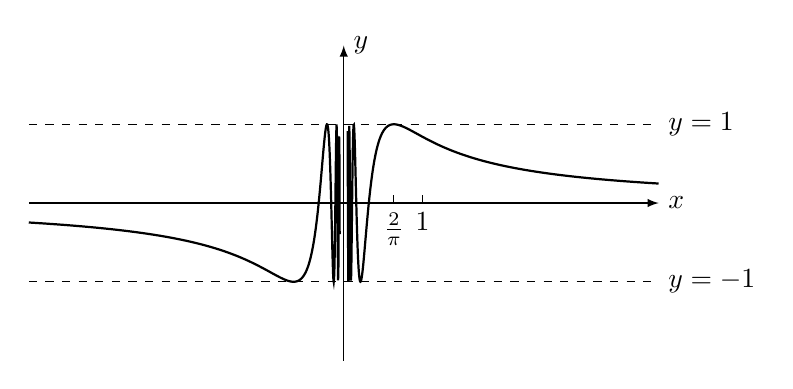
\begin{tikzpicture}[>=latex]
    \draw[->](-4,0)--(4,0)node[right]{$x$};
    \draw[->](0,-2)--(0,2)node[right]{$y$};
    \foreach \x in {1,-1}
    {
        \draw[dashed](-4,\x)--(4,\x)node[right]{$y=\x$};
    }
\draw[domain=-4:-.05, samples=1000, thick]plot(\x, {sin(180/pi/\x)});
\draw[domain=.05:4, samples=1000, thick]plot(\x, {sin(180/pi/\x)});
\foreach \x/\xtext in {1/1, .637/\frac{2}{\pi}}
{
    \draw(\x, 0)node[below]{$\xtext$}--(\x,.1);
}
\end{tikzpicture}    
    \caption{}
\end{figure}

上面是用数列的极限来说明函数的极限,其实我们也可以直接定义函数极限。

\begin{blk}{定义3}
  如果函数$f$在点$a$邻域上有定义(可能去掉点$a$本身),使得当$0<|x-a|<\delta$时,就有$|f(x)-\ell|<\varepsilon$, 那么就说$\ell$为当$x$趋近于$a$时,函数$f$在点$a$的极限值。
\end{blk}

我们对这个定义需要说明以下几点:
\begin{enumerate}
    \item 用定义3验证某数$\ell$是函数$f$在点$a$的极限的办法就是对于任给的$\varepsilon>0$, 要找到这样的正数$\delta$使得能够由不等式$|x-a|<\delta$推出不等式$|f(x)-\ell|<\varepsilon$,虽然$\varepsilon$是任意的正数,但是在找$\delta$的过程中,$\varepsilon$是固定不变的,$\delta$依赖于$\varepsilon$。
    \item 对于已给的$\varepsilon$, 只要证明有一个$\delta>0$存在就行.因为如果有一个$\delta$存在,把$\delta$再缩小一些,显然仍满足我们的要求。
    \item 不等式$|x-a|>0$只是说明$x\ne a$, 即把$x$等于$a$的情况去掉,这是因为我们关心的是函数$f$在点$a$附近的变化趋势,而和函数在$x=a$这点的值无关。
    \item 我们指出定义2和定义3是等价的.
\end{enumerate}

\begin{example}
用定义3证明$\Lim_{x\to 1}\frac{x^3-1}{x-1}=3$
\end{example}

\begin{proof}
    任给$\varepsilon>0$, 要找$\delta>0$, 使由$0<|x-1|<\delta$推出
    $\left|\frac{x^3-1}{x-1}-3\right|<\varepsilon$成立。

    当$x\ne 1$时,
\[\begin{split}
    \left|\frac{x^3-1}{x-1}-3\right|&=|(x^2+x+1)-3|\\
    &=|(x-1)(x+2)|=|x-1|\cdot |x-2|
\end{split}\]

要由$|x-1|\cdot |x+2|<\varepsilon$找$\delta$,显然,这里因子$|x+2|$引起了麻烦。为方便起见,先假定$0<|x-1|<1$,即取$\delta_1=1$,这样
\[0<|x-1|<1\quad\to \quad |x+2|=|(x-1)+3|\le |x-1|+3<4\]因此,要使
\[\begin{cases}
    0<|x-1|<1\\
    |x-1|\cdot |x+2|<\varepsilon
\end{cases}\]
只须
\[\begin{cases}
    0<|x-1|<1\\
    4|x-1|<\varepsilon
\end{cases}\to \quad \begin{cases}
    0<|x-1|<1\\
    |x-1|<\frac{\varepsilon}{4}
\end{cases}\]
由此可见,只须取$\delta=\min\left(1,\frac{\varepsilon}{4}\right)$,即取$\delta$为1与$\frac{\varepsilon}{4}$中的较小者。

$\therefore\quad $对于任意$\varepsilon>0$,取$\delta=\min\left(1,\frac{\varepsilon}{4}\right)$,则当$0<|x-1|<\delta$时,即有
\[\left|\frac{x^3-1}{x-1}-3\right|<\varepsilon\]
这也就证明了
\[\lim_{x\to 1}\frac{x^3-1}{x-1}=3\]
\end{proof}

\begin{example}
    证明$\Lim_{x\to a}\sqrt{x}=\sqrt{a}\quad (a>0)$
\end{example}

\begin{proof}
对于任意的$\varepsilon>0$, 我们必须找到一个$\delta>0$, 使得当$|x-a|<\delta$时,$|\sqrt{x}-\sqrt{a}|<\varepsilon$成立,因为
\[|\sqrt{x}-\sqrt{a}|=\frac{|x-a|}{\sqrt{x}+\sqrt{a}}<\frac{|x-a|}{\sqrt{a}}\]
所以要使$\frac{|x-a|}{\sqrt{a}}<\varepsilon$,只须$|x-a|<\sqrt{a}\varepsilon$

如果取$\delta=\sqrt{a}\varepsilon$,则$\frac{|x-a|}{\sqrt{a}}<\frac{\sqrt{a}\varepsilon}{\sqrt{a}}=\varepsilon$
因此,对于任意$\varepsilon>0$,取$\delta=\sqrt{a}\varepsilon$,则当$|x-a|<\delta$时,就有$|\sqrt{x}-\sqrt{a}|<\varepsilon$成立。这也就证明了
\[\lim_{x\to a}\sqrt{x}=\sqrt{a}\quad (a>0)\]
\end{proof}

有时虽然$f(x)$在某点的左边(或右边)没有定义,如图1.5中的$a,b$两点,我们也可以谈论$f$在点$a$或点$b$两点的极限,譬如对于所有小于$a$的数,$f$虽然没有定义,但是我们可以考察,当$x$从$a$的右侧趋近于$a$时,函数$f$的变化趋势,也就是考察$f$的单边极限是否存在。

\begin{figure}[htp]
    \centering
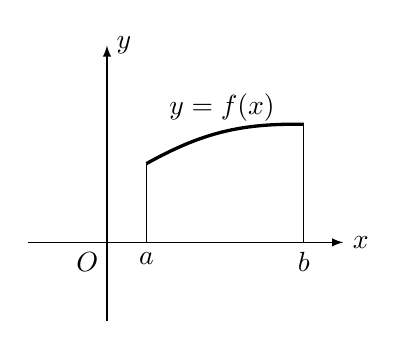
\begin{tikzpicture}[>=latex]
    \draw[->](-1,0)--(3,0)node[right]{$x$};
    \draw[->](0,-1)--(0,2.5)node[right]{$y$};
\draw[very thick](.5,1)to[bend right=-15]node[above]{$y=f(x)$} (2.5,1.5);
\draw(.5,1)--(.5,0)node[below]{$a$};
\draw(2.5,1.5)--(2.5,0)node[below]{$b$};
\node at (-.25,-.25){$O$};
\end{tikzpicture}
    \caption{}
\end{figure}

\begin{blk}{定义}
     设$f(x)$在区间$(a,b)$上有意义,如果任给$\varepsilon>0$, 总存在某个$\delta>0$使得当$x\in (a,a+\delta)$时,总有$|f(x)-\ell|<\varepsilon$,我们就说函数$f$在点$a$以$\ell$为\textbf{右极限},记作:
\[\lim_{x\to a^+}f(x)=\ell\]
\end{blk}

类似地,可以定义\textbf{左极限},只需把开区间$(a,a+\delta)$换成$(b-\delta,b)$就行了,并记作
\[\lim_{x\to b^-} f(x)=\ell\]

\begin{example}
    设函数$f(x)=\begin{cases}
        x-1,&x\le 1\\
x+1,&x>1
    \end{cases}\quad $    
    求$\Lim_{x\to 1^-}f(x)$和$\Lim_{x\to 1^+}f(x)$
\end{example}

\begin{figure}[htp]
    \centering
    \begin{minipage}[t]{0.48\textwidth}
    \centering
    \begin{tikzpicture}[>=stealth, scale=.6]
        \draw[->](-3,0)--(4,0)node[right]{$x$};
        \draw[->](0,-3)--(0,4.5)node[right]{$y$};
        \draw(0,1)node[left]{1}--(.1,1);
        \draw(0,2)node[left]{2}--(.1,2);
        \draw(1,0)node[below]{1}--(1,.1);
        \node at (-.25,-.25){$O$};
        \draw[domain=-2:1, samples=10, very thick]plot(\x,{\x-1});
        \draw[domain=1:3, samples=10, very thick]plot(\x,{\x+1});
    \node at (-2,-3)[left]{$y=x-1$};
    \node at (3,4)[right]{$y=x+1$};
    \draw[dashed](1,0)--(1,2)--(0,2);
    \draw (1,2)[fill=white] circle(2.5pt);
    
    \end{tikzpicture}
    \caption{}
    \end{minipage}
    \begin{minipage}[t]{0.48\textwidth}
    \centering
    \begin{tikzpicture}[>=stealth, scale=.8]
        \draw[->](-3,0)--(4,0)node[right]{$x$};
    \draw[->](0,-2.5)--(0,3)node[right]{$y$};
    \foreach \x in {-2,-1,1,2,3}
    {
        \draw(\x,0)node[below]{$\x$}--(\x,.1);
    }
\foreach \x in {-2,-1,1,2}
{
    \draw(0,\x)--(.1,\x)node[right]{$\x$};
}
\foreach \x in {-2,-1,...,2}
{
    \draw[very thick](\x,\x)--(\x+1,\x);
    \draw (\x+1,\x)[fill=white]circle(2pt);
}
    \node at (.25,-.25){$O$};
    \end{tikzpicture}
    \caption{}
    \end{minipage}
    \end{figure}


\begin{solution}
\[\begin{split}
    \lim_{x\to 1^-}f(x)&=\lim_{x\to 1^-}(x-1)=0\\
    \lim_{x\to 1^+}f(x)&=\lim_{x\to 1^+}(x+1)=2
\end{split}\]
图1.6显示了上面的结果。
\end{solution}

\begin{example}
    函数$y=[x]$代表不超过$x$的最大整数,即若$n\le x<n+1$,$n\in\mathbb{Z}$,则$y=[x]=n$。(图1.7)

求$\Lim_{x\to 2^+}\frac{[x]}{x},\quad \Lim_{x\to 2^-}\frac{[x]}{x}$
\end{example}

\begin{solution}
    显然,当$x=2$时,$\frac{[x]}{x}=\frac{[2]}{2}=\frac{2}{2}=1$, 又
\[\frac{[x]}{x}=\begin{cases}
    \frac{1}{x},& x\in(1,2)\\
    \frac{2}{x},& x\in(2,3)
\end{cases}\]
所以
\[\begin{split}
    \lim_{x\to 2^+}\frac{[x]}{x}&=\lim_{x\to 2^+}\frac{2}{x}=1\\
     \lim_{x\to 2^-}\frac{[x]}{x}&=\lim_{x\to 2^-}\frac{1}{x}=\frac{1}{2}
\end{split}\]    
\end{solution}


下面的命题说明函数的极限与函数的单边极限的关系:

\begin{blk}{定理}
极限$\Lim_{x\to a} f(x)$
存在的必要和充分条件是左极限$\Lim_{x\to a^-} f(x)$和右极限$\Lim_{x\to a^+} f(x)$都存在,并且二者相等。
\end{blk}

\begin{proof}
    必要性
    
    如果$\Lim_{x\to a} f(x)=\ell$, 就是说任给$\varepsilon>0$, 总存在$\delta>0$,
使得当$0<|x-a|<\delta$, 即当$x\in (a-\delta,a)\cup(a,a+\delta)$时,有$|f(x)-\ell|<\varepsilon$。换言之,当$x\in (a-\delta,a)$和$x\in (a,a+\delta)$时,都有$|f (x) -\ell|<\varepsilon$,因此
\[\Lim_{x\to a^-} f(x)=\ell,\qquad \Lim_{x\to a^+} f(x)=\ell\]

充分性

如果$\Lim_{x\to a^-} f(x)=\ell$且$\Lim_{x\to a^+} f(x)=\ell$, 那么总存在$\delta_1>0$, 使得当$x\in(a-\delta_1,a)$时,有
$|f (x) -\ell|<\varepsilon$。

又存在$\delta_2>0$, 使得当$x\in (a,a+\delta_2)$时,有$|f (x) -\ell|<\varepsilon$。

取$\delta=\min(\delta_1,\delta_2)$,于是当$x\in(a-\delta,a+\delta)$时,有$|f (x) -\ell|<\varepsilon$。
这就是说:
\[\Lim_{x\to a} f(x)=\ell\]
\end{proof}

\begin{example}
说明$\Lim_{x\to 3}\frac{|x-3|}{x-3}$是否存在?
\end{example}

\begin{solution}
\[\begin{split}|x-3|&=\begin{cases}
    x-3, & x>3\\
    3-x, &x<3
\end{cases}\\
    \Lim_{x\to 3^-}\frac{|x-3|}{x-3}&=\Lim_{x\to 3^-}\frac{3-x}{x-3}=\Lim_{x\to 3^-}(-1)=-1\\
    \Lim_{x\to 3^+}\frac{|x-3|}{x-3}&=\Lim_{x\to 3^+}\frac{x-3}{x-3}=\Lim_{x\to 3^+}(1)=1
\end{split}\]

$\because\quad \Lim_{x\to 3^-}\frac{|x-3|}{x-3}\ne \Lim_{x\to 3^+}\frac{|x-3|}{x-3}$
    
$\therefore\quad \Lim_{x\to 3}\frac{|x-3|}{x-3}$
不存在。
\end{solution}

\subsection{函数值趋于无穷大}

如果函数$f$在点$a$的邻域上有定义(可能去掉点$a$本身)对于无论多么大的正数$G$, 总存在一个够小的正数$\delta$, 使得当$0<|x-a|<\delta$时,就有$|f(x)|>G$, 那么就说当$x$趋于$a$时,函数$f(x)$趋于\textbf{无穷大},记作
\[\lim_{x\to a} f (x) =\infty\]

\begin{example}
    求证$\Lim_{x\to 0}\frac{1}{x}=\infty$
\end{example}
   
\begin{proof}
设$G$是任意给定的正数,我们要求出一个$\delta>0$, 使得当$|x|<\delta$时,$|f(x)|=\left|\frac{1}{x}\right|>G$。

事实上,要使$\frac{1}{|x|}>G$, 
只须$0<|x|<\frac{1}{G} $。取$\delta=\frac{1}{G}$, 于是当$|x|<\delta$时,就有$\frac{1}{|x|}>G$
因此,
$$\Lim_{x\to 0}\frac{1}{x}=\infty$$
\end{proof}

\begin{example}
    证明当$x\to 0$时,函数$f(x)=\frac{1}{x}\sin\frac{1}{x}\quad (x\ne 0)$不趋于无穷大.
\end{example}

\begin{proof}
如果自变量$x$取数列$\{x_n\}=\left\{\frac{2}{(2n+1)\pi}\Big|n=1, 2, 3,\ldots\right\}$的值趋于0时,$\sin\frac{1}{x}$在原点的任意邻域内无限次交替地取$-1, 1$这两个值,对于这些值,$|f(x)|=\frac{1}{x}=\frac{\pi}{2}(2n+1)$趋于无穷大.

但是当$x$取数列$\{x\}=\left\{\frac{1}{n\pi}\Big| n=1, 2, 3,\ldots\right\}$的
值趋于0时,由于
$\sin\frac{1}{x}=\sin (n\pi) =0$, 
故对于这些值,
$\Lim_{x'_n\to 0} f (x) =0$.

可见在原点的邻近不存在这样的$\delta>0$, 使得当$|x|<\delta$时,$|f(x)|>G$, 因此,当$x\to 0$时,$f(x)=\frac{1}{x}\sin\frac{1}{x}\quad (x\ne 0)$不趋于无穷大.

$y=f(x)$的图象位于两条双曲线$xy=\pm 1$之间,且在原点的邻近作无限多次振动,越靠近原点,曲线的振幅越大(图1.8).

\begin{figure}[htp]
    \centering
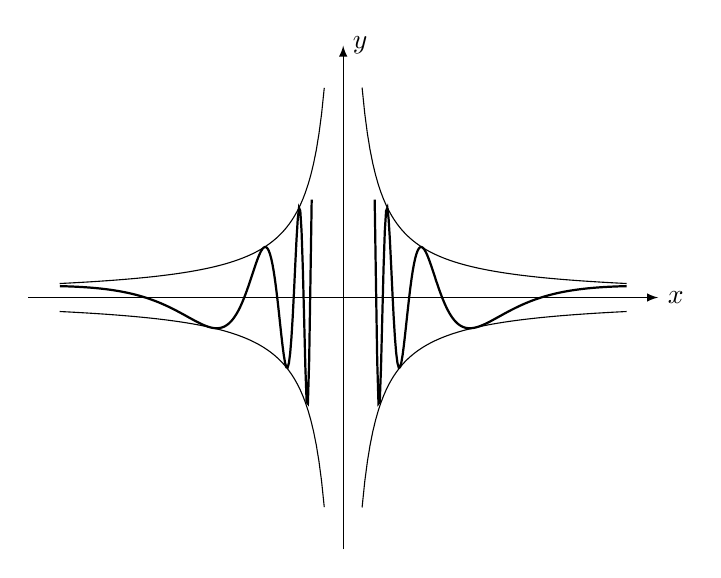
\begin{tikzpicture}[>=latex, scale=.8]
\draw[->](-5,0)--(5,0)node[right]{$x$};
\draw[->](0,-4)--(0,4)node[right]{$y$};
\draw[domain=-4.5:-.3, samples=100]plot(\x,{-1/\x}); 
\draw[domain=-4.5:-.3, samples=100]plot(\x,{1/\x}); 
\draw[domain=.3:4.5, samples=100]plot(\x,{-1/\x}); 
\draw[domain=.3:4.5, samples=100]plot(\x,{1/\x}); 
\draw [domain=.5:4.5, samples=200,  thick]plot(\x, {sin(180/\x*pi)/\x});
\draw [domain=.5:4.5, samples=200,  thick]plot(-\x, {sin(180/\x*pi)/\x});
\end{tikzpicture}
    \caption{}
\end{figure}

\end{proof}

如果对于任何$G>0$, 存在$\delta>0$, 当$0<|x-a|<\delta$时,有$f(x)>G$, 就说当$x\to a$时,函数$f(x)$趋于正无无穷大,记作
\[\lim_{x\to a}f(x)=+\infty\]

如果对于任何$G>0$, 存在$\delta>0$, 当$0<|x-a|<\delta$时,有$f(x)<-G$, 就说当$x\to a$时,函数$f(x)$趋于负无穷大,记作
\[\lim_{x\to a}f(x)=-\infty\]

例如,我们有:
\[\lim_{x\to 0}\frac{1}{x^2}=+\infty,\qquad \lim_{x\to 0}\frac{(-1)}{x^2}=-\infty\]

类似地,我们可以定义:
\[\lim_{x\to a^-}f(x)=+\infty,\quad \lim_{x\to a^+}f(x)=+\infty,\quad \lim_{x\to a^-}f(x)=-\infty,\quad \lim_{x\to a^+}f(x)=-\infty\]
的含义,这里不再写出。建议读者将这些定义严格地写出来。

例如,我们有:
\[\lim_{\theta\to \tfrac{\pi^+}{2}}\tan\theta =+\infty,\qquad \lim_{\theta\to \tfrac{\pi^-}{2}}\tan\theta =-\infty\]
\[\lim_{x\to 0^+}\log_a x =-\infty\quad (a>1),\qquad \lim_{x\to 0^+}\log_a x =+\infty\quad (0<a<1)\]

\begin{ex}
\begin{enumerate}
    \item 用函数极限定义证明:
    \begin{multicols}{2}
        \begin{enumerate}
            \item $\Lim_{x\to \infty}\frac{1}{2x+1}=0$
            \item $\Lim_{x\to 2}x^2=4$
            \item $\Lim_{x\to -1}\frac{x-3}{x^2-9}=\frac{1}{2}$
            \item $\Lim_{x\to 1}\frac{1}{x^2}=1$
            \item $\Lim_{x\to 1}\frac{x^3-x}{x-1}=2$
        \end{enumerate}
    \end{multicols}
    \item 说明:$\Lim_{x\to 3}\frac{x}{x^2-9}=\infty$
    \item 下面极限是否存在?
\begin{multicols}{2}
    \begin{enumerate}
        \item $\Lim_{x\to 1}\frac{2x|x-1|}{x-1}$
        \item $\Lim_{x\to 3}\frac{[x]^2-9}{x^2-9}$
    \end{enumerate}
\end{multicols}
\end{enumerate}
\end{ex}

\subsection{函数极限算法定理}
函数的极限算法定理与数列的极限算法定理类似,因为所谓$\Lim_{x\to a}u(x)=A$, $\Lim_{x\to a}v(x)=B$的意思就是对于任何一个各项都不同于$a$并且以$a$为极限的数列$x_n\to a$, 便有函数值数列$\{u(x_n)\}$, $\{v(x_n)\}$, 并且$\Lim_{n\to \infty}u(x_n)=A$, 
$\Lim_{n\to \infty} v(x_n)=B$, 因此,根据第四册下第三章的定理就可以直接得到相应的结果。现在给出函数的极限运算定理如下:

\begin{blk}{定理}
设$\Lim_{x\to a}u(x)=A$, $\Lim_{x\to a}v(x)=B$,那么
\begin{enumerate}
    \item $\Lim_{x\to a}[u(x)+v(x)]=\Lim_{x\to a}u(x)+\Lim_{x\to a}v(x)$
    \item $\Lim_{x\to a}[u(x)\cdot v(x)]=\Lim_{x\to a} u(x)\cdot \Lim_{x\to a}v(x)$
    \item $\Lim_{x\to a}[c\cdot u(x)]=c\cdot \Lim_{x\to a}u(x)$
    \item $\Lim_{x\to a}\frac{u(x)}{v(x)}=\frac{\Lim_{x\to a}u(x)}{\Lim_{x\to a}v(x)}$ 
    
    只要$v(x)$恒不为0,而且$\Lim_{x\to a}v(x)\ne 0$
    \item $\Lim_{x\to a}\sqrt[n]{u(x)}=\sqrt[n]{\Lim_{x\to a}u(x)}$
    \item 如$\Lim_{x\to a}u(x)=A=\Lim_{x\to a} v(x)$,而$|x-a|<\delta$时,$u(x)<f(x)<v(x)$,则:
    \[\Lim_{x\to a} f(x)=A\]
    即:如果$u(x)$与$v(x)$趋向同一极限$A$,且$f(x)$在$u(x)$与$v(x)$之间,那么,$f(x)$便也趋向那个极限$A$。
\end{enumerate}
\end{blk}

现在只有5需要补证.

设$\Lim_{x\to a}u(x)=A>0$, 则根据函数极限定义:对于$\varepsilon=\frac{A}{2}>0$, 存在$\delta>0$,使得$0<|x-a|<\delta$时,有
\begin{equation}
    u(x)>\frac{A}{2}>0
\end{equation}

于是,
\[\sqrt[n]{u(x)}-\sqrt[n]{A}=\frac{u(x)-A}{\sum^n_{k=1}[u(x)]^{\tfrac{n-k}{n}}A^{\tfrac{k-1}{n}}}\]
由(1.3)式
\[[u(x)]^{\tfrac{n-k}{n}}>\left(\frac{A}{2}\right)^{\tfrac{n-k}{n}}\]
故
\[\begin{split}
    \sum^n_{k=1}[u(x)]^{\tfrac{n-k}{n}}A^{\tfrac{k-1}{n}}&>\sum^n_{k=1}\left(\frac{A}{2}\right)^{\tfrac{n-k}{n}}A^{\tfrac{k-1}{n}}\\
    &=A^{\tfrac{n-1}{n}}\sum^n_{k=1}\left(\frac{1}{2}\right)^{\tfrac{n-k}{n}}\\
    &=A^{\tfrac{n-1}{n}}\left\{\left(\frac{1}{2}\right)^{\tfrac{n-1}{n}}+\left(\frac{1}{2}\right)^{\tfrac{n-2}{n}}+\cdots+\left(\frac{1}{2}\right)^{\tfrac{1}{n}}+1\right\}\\
    &=A^{\tfrac{n-1}{n}}\left\{\frac{1-\left(\frac{1}{2}\right)^{\tfrac{n-1}{n}}\cdot \left(\frac{1}{2}\right)^{\tfrac{1}{n}}}{1-\left(\frac{1}{2}\right)^{\tfrac{1}{n}}}\right\}\\
    &=A^{\tfrac{n-1}{n}}\cdot\frac{\frac{1}{2}}{1-\left(\frac{1}{2}\right)^{\tfrac{1}{n}}}=\frac{A^{\tfrac{n-1}{n}}}{2-2^{\tfrac{n-1}{n}}}\\
\end{split}\]
$\therefore\quad \left|\sqrt[n]{u(x)}-\sqrt[n]{A}\right|<|u(x)-A|\cdot \frac{2-2^{\tfrac{n-1}{n}}}{A^{\tfrac{n-1}{n}}}$

由题设$\Lim_{x\to a}u(x)=A$,而$\frac{2-2^{\tfrac{n-1}{n}}}{A^{\tfrac{n-1}{n}}}$是一个与$x$无关的常数,所以
\[\lim_{x\to a} \sqrt[n]{u(x)}=\sqrt[n]{A}=\sqrt[n]{\lim_{x\to a}u(x)}\]

下面我们来证明两个重要极限公式,为此先介绍一个引理。

\begin{blk}{引理}
     对于任意实数$\theta$, 都有$|\sin\theta|\le |\theta|$
\end{blk}

\begin{proof}
  由于对于任意实数。有$|\sin\theta|\le 1$, 那么仅考虑$\theta\in (0,\pi/2)$即可。
  
  在单位圆$O$上(图1.9),
 截取弧$\wideparen{P_0M}$使弧长$|\wideparen{P_0M}|$等于$\theta$, 其中$P_0$和$M$分别有坐标$(1, 0)$和$(x,y)$, 于是
 \[\sin\theta =y<\sqrt{y^2+ (1-x)^2} =|P_0M|<|\wideparen{P_0M}|=\theta\]
 
 显然,当$\theta=0$时,有$\sin\theta=\theta$. 因此
\[  |\sin\theta | \le |\theta|,\qquad  \theta\in  (0,\pi/2)\]

  如果$-\pi/2<\theta<0$, 则仍有$|MN|<\wideparen{P_0M}$,于是
\[|\sin\theta|<|\theta|,\qquad \theta\in (-\pi/2, 0) \]

  如果$|\theta|\ge \pi/2$, 则因为$\pi/2>1$与$|\sin\theta|\le 1$, 而同样地也得到$|\sin\theta|<|\theta|$. 
  
  因此,对于一切$\theta\ne 0$的值,有$|\sin\theta|<|\theta|$; 当$\theta=0$时,有$|\sin\theta|=|\theta|$。
\end{proof}



\begin{figure}[htp]\centering
    \begin{minipage}[t]{0.48\textwidth}
    \centering
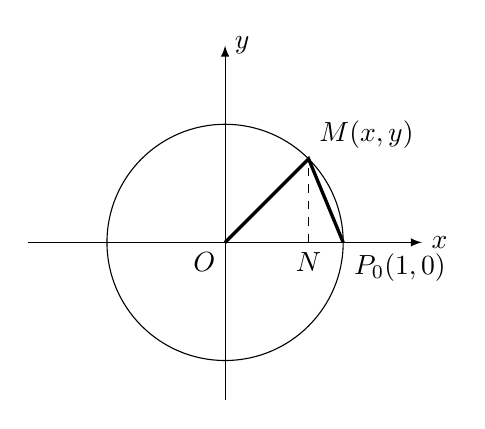
\begin{tikzpicture}[>=latex]
\draw[->](-2.5,0)--(2.5,0)node[right]{$x$};
\draw[->](0,-2)--(0,2.5)node[right]{$y$};
\draw(0,0) circle(1.5);
\draw[very thick](0,0)--(45:1.5)node[above right]{$M(x,y)$}--(1.5,0)node[below right]{$P_0(1,0)$};
\draw[dashed](1.5/1.414,0)node[below]{$N$}--(1.5/1.414,1.5/1.414);
\node at (0,0)[below left]{$O$};
\end{tikzpicture}    
    \caption{}
    \end{minipage}
    \begin{minipage}[t]{0.48\textwidth}
    \centering
    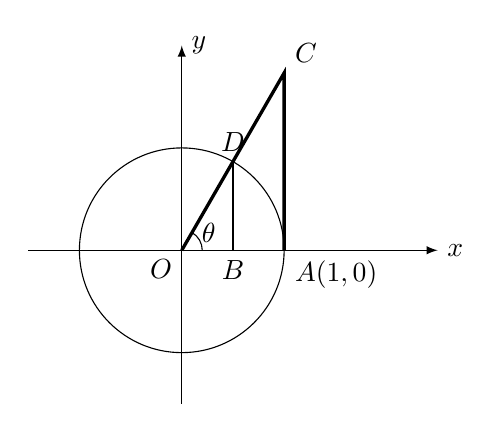
\begin{tikzpicture}[>=latex, scale=1.3]

\draw[->](-1.5,0)--(2.5,0)node[right]{$x$};
\draw[->](0,-1.5)--(0,2)node[right]{$y$};
\draw(0,0) circle(1);
\draw[very thick](0,0)--(60:2)node[above right]{$C$}--(1,0)node[below right]{$A(1,0)$};
\draw[thick](.5,0)node[below]{$B$}--(60:1)node[above]{$D$};
\node at (0,0)[below left]{$O$};   
\draw(0.2,0) arc (0:60:.2)node[right]{$\theta$};   
    \end{tikzpicture}
    \caption{}
    \end{minipage}
    \end{figure}

\begin{blk}{定理}
\[\lim_{\theta\to 0}\frac{\sin\theta }{\theta}=1,\qquad \lim_{\theta\to 0}\frac{\cos\theta-1}{\theta}=0\]
\end{blk}

\begin{proof}
    让我们先证明$\Lim_{\theta\to 0}\frac{\sin\theta }{\theta}=1$。由图1.10容易看出:

假定$\theta$的单位是弧度,于是:
\[\begin{split}
    \triangle OBD\text{的面积}&=\frac{1}{2}OB\cdot BD=\frac{1}{2}\cos\theta\cdot \sin\theta\\
    \triangle OAC\text{的面积}&=\frac{1}{2}OA\cdot AC=\frac{1}{2}\cdot 1\cdot \tan\theta\\
    \text{扇形$OAD$的面积}&=\frac{1}{2}OA\cdot \wideparen{AD}=\frac{1}{2}\cdot 1^2\cdot \theta
\end{split}\]

假如角是用180等分平角的“度”作为单位,则扇形面积就是$\frac{1}{2}\cdot 1\cdot \frac{\pi}{100}\theta$。

因为上述扇形是夹在$\triangle OBD$和$\triangle OAC$之间,所以
\begin{equation}
    \frac{1}{2}\cos\theta\sin\theta<\frac{1}{2}\theta<\frac{1}{2}\tan\theta=\frac{1}{2}\frac{\sin\theta}{\cos\theta}
\end{equation}
即有,若$0<\theta<\frac{\pi}{2}$,则
\begin{equation}
    \cos\theta<\frac{\sin\theta}{\theta}<\frac{1}{\cos\theta}
\end{equation}
注意到:$\sin(-\theta)=-\sin\theta$和$\cos(-\theta)=\cos\theta$, 不等式(1.5)也蕴含,若$-\frac{\pi}{2}<\theta<0$, 则
\begin{equation}
    \cos(-\theta)<\frac{\sin(-\theta)}{-\theta}<\frac{1}{\cos(-\theta)}
\end{equation}
将不等式(1.5)和(1.6)合并为,若$0<|\theta|<\frac{\pi}{2}$,则
\begin{equation}
    \cos\theta<\frac{\sin\theta}{\theta}<\frac{1}{\cos\theta}
\end{equation}
又因为
\[0\le |1-\cos\theta|=\left|2\sin^2\frac{\theta}{2}\right|\le 2\left|\sin\frac{\theta}{2}\right|<|\theta|\]
从而
\[0\le \lim_{\theta\to 0}|1-\cos\theta|\le \lim_{\theta\to 0}|\theta|=0\]
所以
\[\lim_{\theta\to 0}|1-\cos\theta|=0\]
即:$\Lim_{\theta\to 0}\cos\theta=1$
由(1.7)知被夹逼在两者之间的$\frac{\sin\theta}{\theta}$极限值也就一定是1了!

以$\Lim_{\theta\to 0}\frac{\sin\theta}{\theta}=1$为基础,则:
\[\begin{split}
\lim_{\theta\to 0}\frac{\cos\theta-1}{\theta}&=\lim_{\theta\to 0}\left\{\frac{-2\left(\sin\frac{\theta}{2}\right)^2}{\theta}\right\}\\
&= \lim_{\theta\to 0}\left(-\sin\frac{\theta}{2}\right)\frac{\sin\frac{\theta}{2}}{\frac{\theta}{2}}    \\
&=\lim_{\theta\to 0}\left(-\sin\frac{\theta}{2}\right)\cdot \lim_{\theta\to 0}\frac{\sin\frac{\theta}{2}}{\frac{\theta}{2}}   \\
&=0\cdot 1=0
\end{split}   
\]
\end{proof}

\begin{example}
求:$\Lim_{x\to 2}\frac{x^2+3x-10}{3x^2-5x-2},\qquad \Lim_{x\to 0}\frac{\sqrt[3]{1+x^2}-1}{x^2}$
\end{example}

\begin{solution}
    如果应用前面的定理去分别求两式中的分子、分母的极限时,其分子、分母的极限值均为零,即我们得到$\frac{0}{0}$的不定形式。我们通常要对原代数式变形,找出分子、分母中具有$x-a$的因子,消去$x-a$的公共因子,一般问题就可解决。
\[\begin{split}
    \Lim_{x\to 2}\frac{x^2+3x-10}{3x^2-5x-2}&=\Lim_{x\to 2}\frac{(x+5)(x-2)}{(3x+1)(x-2)}\\
    &=\Lim_{x\to 2}\frac{x+5}{3x+1}\\
    &=\frac{2+5}{3\x 2+1}=1
\end{split}\]

\[\begin{split}
    \Lim_{x\to 0}\frac{\sqrt[3]{1+x^2}-1}{x^2}&=\Lim_{x\to 0}\frac{{(1+x^2)}-1}{x^2\left(\sqrt[3]{(1+x^2)^2}+\sqrt[3]{1+x^2}+1\right)}\\
    &=\Lim_{x\to 0}\frac{1}{\sqrt[3]{(1+x^2)^2}+\sqrt[3]{1+x^2}+1}=\frac{1}{3}
\end{split}\]
\end{solution}

\begin{example}
    求:$\Lim_{x\to 0}\frac{\cos x-1}{x^2},\qquad \Lim_{x\to \pi}\frac{\sin mx}{\sin nx}(m,n\in \mathbb{N})$
\end{example}

\begin{solution}
\[\begin{split}
    \Lim_{x\to 0}\frac{\cos x-1}{x^2}&=\Lim_{x\to 0}\frac{-2\left(\sin\frac{x}{2}\right)^2}{x^2}\\
    &=\frac{-2}{2^2}\Lim_{x\to 0}\frac{\sin\frac{x}{2}}{\frac{x}{2}}\cdot \Lim_{x\to 0}\frac{\sin\frac{x}{2}}{\frac{x}{2}}\\
    &=\left(-\frac{1}{2}\right)\cdot 1\cdot 1=-\frac{1}{2}
\end{split}\]

由三角函数诱导公式易知
\[\sin m(\pi-x)=\sin(m\pi-mx)=(-1)^{m-1}\sin mx\]
同样得到
\[\sin n(\pi-x)=(-1)^{n-1}\sin nx\]
因此:
\[(-1)^{m-n}\frac{\sin mx}{\sin nx}=\frac{\sin m(\pi-x)}{\sin n(\pi-x)}\]
两边乘以$(-1)^{m-n}$,得
\[\frac{\sin mx}{\sin nx}=(-1)^{m-n}\frac{\sin m(\pi-x)}{\sin n(\pi-x)}\]
设$y=\pi-x$, 则当$x\to \pi$, 有$y\to 0$, $my\to 0$, $ny\to 0$. 因此:
\[\begin{split}
    \Lim_{x\to \pi}\frac{\sin mx}{\sin nx}&=\lim_{y\to 0}(-1)^{m-n}\frac{\sin my}{\sin ny}\\
&=(-1)^{m-n}\lim_{y\to 0}\left(\frac{m}{n}\cdot \frac{\sin my}{my}\cdot \frac{ny}{\sin ny}\right)\\
&=(-1)^{m-n}\cdot \frac{m}{n}\cdot 1\cdot 1=(-1)^{m-n}\frac{m}{n}
\end{split}\]
\end{solution}

\begin{example}
由条件$\Lim_{x\to -\infty}\left(\sqrt[]{x^2-x+1}-ax-b\right)=0$,求出$a,b$的值。
\end{example}

\begin{solution}
$\because\quad \Lim_{x\to -\infty}\left(\sqrt{x^2-x+1}-ax-b\right)=0,\quad \Lim_{x\to -\infty}\frac{1}{x}=0$

$\therefore\quad \Lim_{x\to -\infty}\left(\sqrt{x^2-x+1}-ax-b\right)\cdot \frac{1}{x}=0$

即:
\[\Lim_{x\to -\infty}\left(\frac{\sqrt{x^2-x+1}}{x}-a-\frac{b}{x}\right)=0\]
又因为:当$x<0$时,
\[\sqrt{x^2-x+1}=\sqrt{x^2\left(1-\frac{1}{x}+\frac{1}{x^2}\right)}=-x\sqrt{1-\frac{1}{x}+\frac{1}{x^2}}\]
所以上式可写成
\[\lim_{x\to -\infty}\left(-\sqrt{1-\frac{1}{x}+\frac{1}{x^2}}-a-\frac{b}{x}\right)=0\]
即:$-1-a-0=0\quad \to \quad a=-1$

代入原条件,得
\[\lim_{x\to -\infty}\left(\sqrt{x^2-x+1}+x-b\right)=0\]
即:
\[\begin{split}
    b&=\lim_{x\to-\infty}\left(\sqrt{x^2-x+1}+x\right)\\
    &=\lim_{x\to-\infty} \frac{x^2-x+1-x^2}{\sqrt{x^2-x+1}-x}  \\
    &=\lim_{x\to-\infty}\frac{-x\left(1-\frac{1}{x}\right)}{-x\left(\sqrt{1-\frac{1}{x}+\frac{1}{x^2}}+1\right)}    \\
    &=\lim_{x\to-\infty}\frac{1-\frac{1}{x}}{\sqrt{1-\frac{1}{x}+\frac{1}{x^2}}+1} =\frac{1}{2}   \\
\end{split}\]

$\therefore\quad a=-1,\quad b=\frac{1}{2}$为所求。
\end{solution}

\begin{ex}
\begin{enumerate}
    \item 说明当$x\to \infty$时,函数$\frac{x^5-4}{x^3+x}$的变化趋势。
    \item 求极限
    \begin{enumerate}
\begin{multicols}{2}
    \item  $\Lim _{x \to 0} \frac{(x+2)^{2}}{x^{2}+4}$
    \item  $\Lim _{x \to 2} \frac{x^{2}-4}{x-2}$
    \item  $\Lim _{x \to 2} \frac{5 x^{2}+x-8}{x^{2}-4}$
    \item  $\Lim _{x \to 0} \frac{\left(4 x^{3}-3\right)(1-2 x)}{7 x^{3}-6 x+4}$
    \item  $\Lim _{x \to \infty} \frac{3 x^{5}}{x^{5}-x^{2}+1}$
    \item  $\Lim _{x \to \infty} \frac{\left(x^{2}-5\right)\left(x^{2}+7\right)}{x^{4}+35}$
    \item  $\Lim _{x \to 3} \frac{x^{2}-8 x+15}{x^{2}-7 x+12}$
    \item  $\Lim _{x \to -3} \frac{x^{2}-9}{x^{2}+9 x+18}$
    \item $\Lim _{x \to -1} \frac{x\left(x^{2}+4 x+3\right)}{x^{3}+3 x^{2}+5 x+3}$
    \item  $\Lim _{x \to 1} \frac{x^{3}+x^{2}-2}{x^{4}+2 x^{2}-2 x-1}$
    \item $\Lim _{x \to \infty} \frac{x+\sin x}{2 x+5}$
    \item  $\Lim _{x \to 0} \frac{(1+x)^{5}-(1+5 x)}{x^{2}+x^{5}}$
\end{multicols}
    \item  $\Lim _{x \to 0} \frac{(1+m x)^{n}-(1+n x)^{m}}{x^{2}}\qquad (m, n \in \mathbb{N})$
    \item  $\Lim _{x \to 1} \frac{x^{2}+x^{4}+\cdots+x^{2 n}-n}{x-1}$
\end{enumerate}

    \item 求极限  
\begin{enumerate}
\begin{multicols}{2}
\item $\Lim_{x\to 0^+}\sqrt{3x} $
\item $\Lim_{x\to 1^-}\sqrt{1-x} $
\item $\Lim_{x\to 3^-} 3[x]$
\item $\Lim_{x\to 1^+} [x+3]$
\item $\Lim_{x\to -3^+}\left(1+\sqrt{x+3}\right) $
\item $\Lim_{x\to 4^-} \left(\sqrt{4-x}+[x-1]\right)$
    \item $\Lim_{x\to 1^+}\frac{2x|x-1|}{x-1} $
    \item $\Lim_{x\to 4^-} ([x]-x)$
\end{multicols}
    \item $\Lim_{x\to 0^+}\frac{b}{x}\left[\frac{x}{a}\right] \qquad (a>0,\; b>0)$
    \item $\Lim_{x\to 0^+} \frac{x}{a}\left[\frac{b}{x}\right]\qquad (a>0,\; b>0)$
\end{enumerate}    

    \item 求极限  
\begin{enumerate}
\begin{multicols}{2}
\item $\Lim _{x \to  1} \frac{1-x}{\sqrt{1-x^{2}}}$;
\item  $\Lim _{x \to  1} \frac{1-\sqrt{x}}{1-x}$;
\item  $\Lim _{x \to  1} \frac{(2 x-3)(\sqrt{x}-1)}{2 x^{2}+x-3}$
\item  $\Lim _{x \to  2} \frac{x-2}{\sqrt{x^{2}-2}-\sqrt{2}}$
\item  $\Lim _{t \to +\infty}(\sqrt{1+t}-\sqrt{t})$;
\item  $\Lim _{x \to +\infty} \sqrt{x}(\sqrt{x+a}-\sqrt{x})$
\item  $\Lim _{x \to  5} \frac{\sqrt{x-1}-2}{x-5}$;
\item $\Lim _{x \to  0} \frac{\sqrt[3]{1+x}-\sqrt[3]{1-x}}{x}$
\item  $\Lim _{x \to  1} \frac{4 x+\sqrt{x-1}}{2 x-\sqrt{x+1}}$
\item  $\Lim _{x \to  1} \frac{x-1}{\sqrt{x^{2}-1}+\sqrt{x-1}}$
\item $\Lim _{x \to  a} \frac{\sqrt{x-a}+\sqrt{x}-\sqrt{a}}{\sqrt{x^{2}-a^{2}}}$
\item  $\Lim _{x \to -\infty} \frac{x-2}{\sqrt{x^{2}-4 x+3}}$
\item $\Lim _{x \to -\infty}\left[\frac{2(x-1)^{2}}{\sqrt{4 x^{2}+2 x+1}}+x\right]$
\end{multicols}
\item $\Lim _{x \to +\infty}\left(\sqrt{x+\sqrt{x+\sqrt{x}}}-\sqrt{x}\right)$
\item $\Lim _{x \to +\infty} x\left(\sqrt{x^{2}+2 x}-2 \sqrt{x^{2}+x}+x\right)$
\end{enumerate}   

\item \begin{enumerate}
    \item $f(x)=\begin{cases}
        0,& x>1\\
        1,& x=1\\
        x^2+2, &x<1
    \end{cases}$

    求$f(x)$在$x=1$的左右极限。

    \item $f(x)=\begin{cases}
        x\sin\frac{1}{x},& x>0\\
        1+x^2,& x<0
    \end{cases}$

    求$f(x)$在$x=0$的左右极限。

    \item $\Lim_{x\to 3}\frac{[x]^2-9}{x^2-9}$是否存在?
    \item $\Lim_{x\to 0}\frac{x}{|x|}$是否存在?
\end{enumerate}

\item 若$0<x<\frac{\pi}{2}$,求证:
\begin{multicols}{2}
    \begin{enumerate}
        \item $\tan x>x$
        \item $x-\frac{x^2}{4}<\sin x<x$
    \end{enumerate}
\end{multicols}

\item 求极限  
\begin{enumerate}
\begin{multicols}{2}
    \item $\Lim_{x\to 0} \frac{\sin ax}{x}$
    \item $\Lim_{x\to 0} \frac{\sin 7x}{4x}$
    \item $\Lim_{\theta\to 0} \frac{\sec2\theta\sin\theta}{\theta}$
    \item $\Lim_{\theta \to 0} \frac{\tan\theta}{\theta}$
    \item $\Lim_{t\to 0} \frac{15t}{\tan 6t}$
    \item $\Lim_{x\to 0} \frac{\tan 2x}{\sin 7x}$
    \item $\Lim_{\theta \to 0} \frac{\tan\theta-\sin\theta}{\theta^2}$
    \item $\Lim_{x\to 0} \frac{\csc x-\cot x}{x}$
    \item $\Lim_{x\to 0} \frac{\sin^2\frac{x}{2}}{x^2}$
    \item $\Lim_{x\to \pi} \frac{\sin x}{\pi-x}$
    \item $\Lim_{x\to 1} \frac{1+\cos\pi x}{\tan^2 \pi x}$
    \item $\Lim_{x\to \tfrac{\pi}{4}}\tan 2x\tan\left(\frac{\pi}{4}-x\right) $ 
    \item $\Lim_{x\to 1} (1-x)\tan\frac{\pi x}{2}$
    \item $\Lim_{x\to 0} \frac{\sin mx}{\sin nx}$
    \item $\Lim_{x\to 0} \frac{x+\sin x}{x+2\sin x}$
    \item $\Lim_{x\to 0} \frac{\sqrt{\cos x}-1}{x^2}$
\end{multicols}
\end{enumerate}   

\end{enumerate}
\end{ex}

\subsection{数$e$}
我们在这里要利用数列的极限来定义一个新的数,这一个数不论对于分析本身或者对于它的应用来说都是非常重要的。

考虑数列$a_n=\left(1+\frac{1}{n}\right)^n,\; n=1, 2, 3,\ldots$的极限.

首先我们计算一下数列$\{a_N\}$的数值:
\begin{center}
\begin{tabular}{llll}
   $a_1=2.0$ & $a_2=2.250$ & $a_3=2.370$& $a_4=2.441$\\
$a_5=2.488$ &$a_6=2.522$& $a_7=2.546$& $a_8=2.565$\\
$\cdots$ &$a_{256}=2.712$&$\cdots$&$a_{1024}=2.717$\\ 
\end{tabular}
\end{center}

观察这一串数,我们会猜测这个数列是递增的,可能收敛于一个极限值,现在我们来证明这个猜想成立。

依牛顿二项式定理,即有















\begin{example}
    
\end{example}


\begin{solution}
    
\end{solution}


\begin{example}
    
\end{example}

\begin{solution}
    
\end{solution}

\begin{example}
    
\end{example}

\begin{solution}
    
\end{solution}

\begin{solution}
    
\end{solution}






\begin{solution}
    
\end{solution}


























































































